\chapter{\ifenglish Background Knowledge and Theory\else ทฤษฎีที่เกี่ยวข้อง\fi}

การทําโครงงานให้มีความสําเร็จเเละมีความสมบูรณ์ จําเป็นต้องศึกษาค้นคว้าทฤษฎีที่เกี่ยวข้อง ซึ่งเนื้อหาในบทนี้จะเกี่ยวกับการอธิบายถึงสิ่งที่เกี่ยวข้องกับโครงงาน เพื่อให้ผู้อ่านเข้าใจเนื้อหาในบทถัดไปได้ง่ายมากขึ้น โดยจะเเบ่งเนื้อหาหลักออกมาได้ดังนี้


\section{HTML (Hypertext Markup Language)}

{HTML ย่อมาจาก Hypertext Markup Language เป็นภาษาที่ใช้ในการ  แสดงผลในเว็บบราวเซอร์บนอินเตอร์เน็ต สามารถแสดงข้อมูลตัวอักษร ภาพ, เสียง และไฟล์ในรูปแบบอื่นๆ โดยโครงสร้างหลักของ HTML ก็จะเริ่มด้วย <html> และจบด้วย </html> เสมอ เเละยังมี <tag> ต่างๆที่หลากหลายให้ใช้งานตามความต้องการ ซึ่งชุดคำสั่งที่ใช้จะแยกเป็น 2 ส่วนคือ}

\begin{enumerate}
  \item head คำสั่งที่อยู่ในส่วนนี้จะใช้อธิบายรายละเอียดเกี่ยวกับ web page จะแสดงผลที่ web page โดยตรง 
  \item body คำสั่งที่อยู่ในส่วนนี้จะใช้ในการจัดรูปแบบตัวอักษร จัดหน้า ใส่รูปภาพ ซึ่งตัวอักษร ในส่วนนี้จะแสดงที่ web browser โดยตรงเช่น ข้อความ, รูปภาพ, เสียง, วีดิโอ หรือไฟล์ต่างๆ
  
\end{enumerate}

\section{JavaScript}

ภาษา JavaScript เป็นภาษาเขียนโปรแกรมที่ถูกพัฒนาและปฏิบัติตามข้อกำหนดมาตรฐานของ ECMAScript ภาษา JavaScript นั้นเป็นภาษาระดับสูง คอมไพล์ในขณะที่โปรแกรมรัน (JIT) และเป็นภาษาเขียนโปรแกรมแบบหลายกระบวนทัศน์ เช่น การเขียนโปรแกรมเชิงขั้นตอน การเขียนโปรแกรมเชิงวัตถุ หรือการเขียนโปรแกรมแบบ Functional ภาษา JavaScript มีไวยากรณ์ที่เหมือนกับภาษา C ใช้วงเล็บเพื่อกำหนดบล็อคของคำสั่ง นอกจากนี้ JavaScript ยังเป็นภาษาที่มีประเภทข้อมูลแบบไดนามิกส์ เป็นภาษาแบบ Prototype-based และ First-class function เเละยังถือว่าเป็นเทคโนโลยีหลักของการพัฒนาเว็บไซต์ ทำให้หน้าเว็บสามารถตอบโต้กับผู้ใช้ได้โดยที่ไม่จำเป็นต้องรีเฟรชหน้าใหม่ (Dynamic website) เนื่องจากภาษา JavaScript เป็นภาษาเขียนโปรแกรมแบบหลายกระบวนทัศน์ ทำให้สามารถรองรับการเขียนโปรแกรมทั้งแบบ Event-driven, Functional และแบบลำดับขั้นตอน รวมไปถึง Javascript ยังมีไลบรารี่ APIs สำหรับร่วมทำงานกับ Document Object Model (DOM) ซึ่งเป็น API ที่โดยทั่วไปแล้วสามารถพบได้บนเว็บเบราว์เซอร์ซึ่งในโครงงานนี้ ผู้พัฒนาได้ใช้ Library และ Framwork ของ Javascript ตามลำดับต่อไปนี้ 


\subsection{React (Front-end)}

React เป็น JavaScript Library โดยสร้างมาจากพื้นฐานแนวความคิดแบบ MVC(Model View Controller) ซึ่งหมายถึงว่า React มีหน้าที่จัดการกับ Model หรือ View (UI) ซึ่งรองรับการเขียนด้วย JSX (JavaScript syntax extension) เเละ Typescript โดยหลักการเขียนนั้นมีพื้นฐานประกอบมาจาก javascript เเละ html ผู้ใช้งานจึงต้องมีพื้นฐานื เช่นการเขียน Component นั้น ก็เหมือนกับการเขียน HTML เเต่  React ใช้สิ่งที่เรียกว่า JSX ในการแสดงผลเว็บไซต์ หน้าตาจะคล้ายคลึง HTML มาก แตกต่างตรงเราเขียนเข้าไปในไฟล์ JavaScript แทนไฟล์ HTML ทำให้เราสามารถใส่ลูกเล่นอะไรกับมันได้มากกว่า จะเห็นว่าจริง ๆ แล้ว React มีความคล้ายกับ HTML ที่เราเขียนกันปกติอยู่แล้วมาก โดยสรุปคือ คอนเซปต์ที่เราต้องรู้เพื่อเขียน React มี 3 Concept ได้เเก่


\begin{enumerate}
  \item Component – ส่วนต่าง ๆ ในเว็บเราจะมองเป็น Component
  \item State – ข้อมูลที่อยู่ใน Component แต่ละชิ้น เราเรียกว่า State
  \item Props – ข้อมูลที่ถูกส่งต่อจาก Component ชั้นบนลงไปชั้นล่าง เราเรียกว่า Props (Properties)
\end{enumerate}

\subsubsection{ NodeJS (Express) (Back-end)}

Express.js หรือ Express นั้นเป็นเว็บเฟรมเวิร์คจาก NPM (Node Package Manager) ที่ใช้สำหรับพัฒนาเว็บแอพพลิเคชันหรือเว็บไซต์บน Node.js ที่ทำงานที่ฝั่งของ Backend ตัวของเฟรมเวิร์คนั้นถูกพัฒนามาจากโมดูล http ซึ่งเป็นโมดูลของ Node.js เอง แต่เราใช้มันเพื่อทำให้การพัฒนาเว็บแอพพลิเคชันบน Node.js ทำได้ง่ายขึ้น และ Express.js มีคุณสมบัติที่โดดเด่นคือ

\begin{enumerate}
  \item การจัดการ Routing ที่ง่าย
	\item ฟังก์ชันช่วยสำหรับ HTTP
	\item สนับสนุน Template engines สำหรับสร้าง View
	\item ทำงานได้รวดเร็วและมีประสิทธิภาพ
	\item สนับสนุน Middleware
\end{enumerate}



\section{GraphQL}

GraphQL คือ ภาษาสำหรับการเข้าถึงข้อมูล (Query Language) เพื่อการใช้งาน API ของระบบและประมวลผลคำสั่งที่ฝั่ง server หรือที่เรียกว่า server-side runtime โดยใช้โครงสร้างข้อมูลที่เรากำหนดไว้ มีคุณสมบัติ ที่ใช้งาน เข้าใจง่าย ไม่ซับซ้อน และให้ผลลัพธ์ได้ตรงตามความต้องการของผู้ใช้งาน การใช้ GraphQL สามารถจัดการเพียงแค่ข้อมูลที่เราต้องการใช้ออกมา ทำให้เราสามารถปรับเปลี่ยน (customize) รูปแบบของข้อมูลที่เราจะนำไปใช้ต่อได้ตามต้องการ ด้วยการสืบค้น (Query) และเปลี่ยนแปลง (Mutate) ข้อมูล ซึ่งเป็นวิธีการหลัก ของ GraphQLโดยไม่ยุ่งยาก ส่งผลให้ข้อมูลที่ได้จากฐานข้อมูลมีประสิทธิภาพมากขึ้น ผ่านหลักการคือ หลังจากเราส่ง request เพื่อไปดึงข้อมูลมาจาก API ผลลัพธ์ที่ได้จะถูกส่งกลับมาในรูปแบบของ JSON (JavaScript Object Notation) ทําให้เราสามารถใช้ข้อมูลในรูปแบบที่เเตกต่างในสถานการณ์ที่หลากหลายได้ เช่น บน Web platform เราต้องการใช้ข้อมูลทั้งหมด ในขณะที่บน Mobile platform ทพื้นที่ (space) จำกัด เราอาจจะต้องการใช้ข้อมูลเพียงบางส่วน ทําให้ในปัจจุบันถูกนำไปใช้งานอย่างแพร่หลายในหลายบริษัทชั้นนํา

\section{NoSQL (MOngoDB)}

ฐานข้อมูล NoSQL สร้างตามวัตถุประสงค์สำหรับโมเดลข้อมูลแบบเฉพาะเจาะจงและมีแบบแผนที่ยืดหยุ่น เเละเป็นที่รู้จักกันดีในด้านความง่ายในการพัฒนา การทำงาน และประสิทธิภาพตามขนาดที่ต้องการ มีการใช้โมเดลข้อมูลที่หลากหลายสำหรับการเข้าถึงและจัดการข้อมูล ฐานข้อมูลประเภทนี้ได้รับการปรับปรุงประสิทธิภาพสำหรับแอปพลิเคชันที่ต้องใช้ข้อมูลปริมาณมาก มีเวลาแฝงต่ำ ซึ่งเกิดขึ้นโดยการผ่อนปรนข้อจำกัดความสม่ำเสมอข้อมูลของฐานข้อมูลอื่นๆ ฐานข้อมูล NoSQL เหมาะสมมากสำหรับแอปพลิเคชันสมัยใหม่ เช่น อุปกรณ์เคลื่อนที่ เว็บ และเกมที่จำเป็นต้องมีฐานข้อมูลที่ปรับขนาดได้ ประสิทธิภาพสูง และทำงานได้ดีเยี่ยมเพื่อมอบประสบการณ์ผู้ใช้ที่ยอดเยี่ยม 
คุณสมบัติที่สําคัญเเละรายละเอียดของ NOSQL

\begin{enumerate}
  \item ความยืดหยุ่น: มีแบบแผนยืดหยุ่นที่ทำให้การพัฒนาเกิดขึ้นเร็วและทำซ้ำคำสั่งได้ดียิ่งขึ้นกว่าเดิม โมเดลข้อมูลที่ยืดหยุ่นทำให้ฐานข้อมูล NoSQL เหมาะสมที่สุดสำหรับข้อมูลแบบกึ่งมีโครงสร้างและไม่มีโครงสร้าง

  \item ความสามารถในการปรับขนาด: ปรับขนาดออกได้โดยใช้คลัสเตอร์แบบกระจายของฮาร์ดแวร์แทนการปรับขนาดขึ้นโดยเพิ่มเซิร์ฟเวอร์ที่มีราคาแพงและมีประสิทธิภาพสูง ผู้ให้บริการระบบคลาวด์บางเจ้าจัดการปฏิบัติการนี้อยู่เบื้องหลังในแบบบริการที่มีการจัดการเต็มรูปแบบ

  \item ประสิทธิภาพสูง: ฐานข้อมูล NoSQL ได้รับการปรับปรุงประสิทธิภาพสำหรับโมเดลข้อมูลบางโมเดล และเข้าถึงรูปแบบที่เปิดใช้งานประสิทธิภาพที่สูงกว่าการพยายามดำเนินการทำงานที่คล้ายกันด้วยฐานข้อมูลเชิงสัมพันธ์

  \item  ทำงานได้ดีเยี่ยม: ฐานข้อมูล NoSQL มี API การทำงานและประเภทข้อมูลที่สร้างตามวัตถุประสงค์สำหรับโมเดลข้อมูลแต่ละโมเดลที่สอดคล้องกัน
\end{enumerate}


NoSQL ที่เราเลือกใช้จะเป็นของ MongoDB ซึ่งเป็นฐานข้อมูลรูปเเบบเอกสาร (Document store) ที่มีประสิทธิภาพสูง ใช้ง่ายง่าย ถูกใช้อย่างเเพร่หลาย เหมาะสมสําหรับโครงงานนี้

\subsubsection{ MongoDB}


MongoDB เป็นฐานข้อมูลเอกสารที่ได้รับความนิยม ซึ่งช่วยให้ API มีประสิทธิภาพและใช้งานง่ายสำหรับการพัฒนาที่ยืดหยุ่นและมีการทำซ้ำ ของข้อมูล ในโค้ดแอปพลิเคชันมักจะมีการแสดงข้อมูลเป็นวัตถุ หรือเอกสารที่เป็น BSON ซึ่งเป็นโมเดลข้อมูลที่มีประสิทธิภาพและใช้งานง่ายสำหรับ Developer ฐานข้อมูลแบบเอกสารยังช่วยให้ Developer จัดเก็บและสืบค้นข้อมูลในฐานข้อมูลได้ง่ายขึ้น โดยใช้รูปแบบโมเดลเอกสารเดียวกันที่ใช้ในโค้ดแอปพลิเคชัน 

\section{การคํานวณเกรด}

การคำนวณเกรดเฉลี่ยจะใช้สูตรคำนวณต่อไปนี้
\[\mathrm{GPA}=\frac{\sum_{i=1}^{n}{G_i\cdot P_i}}{\sum_{i=1}^{n}{P_i}}\]
โดยที่
\begin{itemize}
\item $\mathrm{GPA}$ คือเกรดเฉลี่ยโดยรวม 
\item $G_i$ คือเกรดที่ได้ในวิชาที่ $i$
\item $P_i$ คือหน่วยกิจที่ได้ในวิชาที่ $i$
\item $n$ คือจำนวนวิชา
\end{itemize}
โดยมหาวิทยาลัยเชียงใหม่ เกรด G จะมีดังนี้ 

\begin{figure}
  \begin{center}
  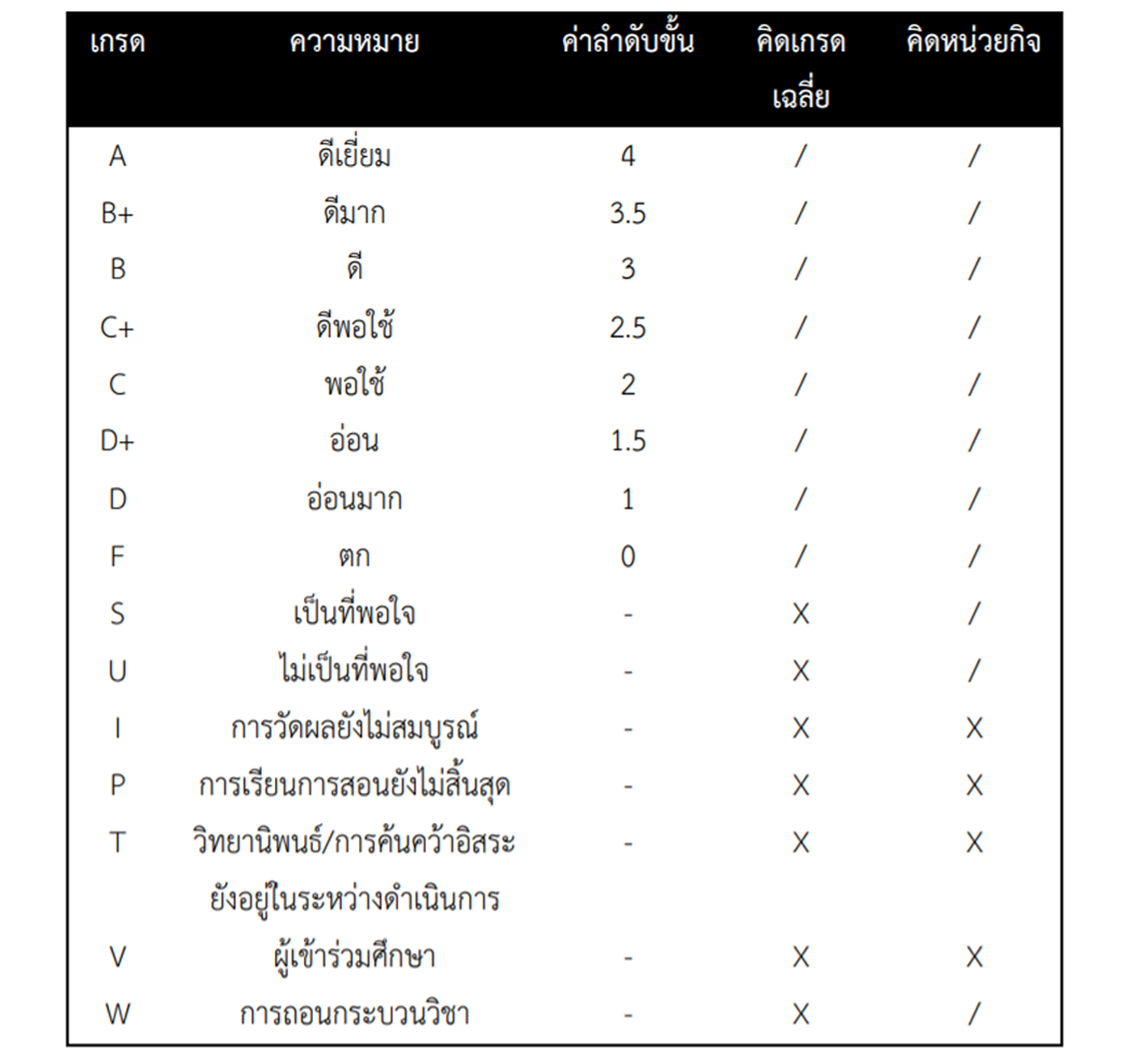
\includegraphics[width=1\textwidth]{table.png}
  \end{center}
  \caption {ตารางเเสดงเกรด}
  \end{figure}

\section{
เกณฑ์มาตรฐานหลักสูตรระดับปริญญาตรี พ.ศ. 2558 ตามประกาศของกระทรวงศึกษาธิการ
}

-โครงสร้างหลักสูตร

โดยตามประกาศของกระทรวงศึกษาธิการได้กล่าวถึงโครงสร้างของหลักสูตรในระดับปริญญาตรีไว้ดังนี้ว่า โครงสร้างหลักสูตร ต้องประกอบด้วยหมวดวิชาศึกษาทั่วไป หมวดวิชาเฉพาะ และหมวดวิชาเลือกเสรี โดยมีสัดส่วนจํานวนหน่วยกิตของแต่ละหมวดวิชา ดังนี้
\begin{enumerate}
    \item หมวดวิชาศึกษาทั่วไป หมายถึง หมวดวิชาที่เสริมสร้างความเป็นมนุษย์ที่สมบูรณ์ ให้มีความรอบรู้อย่างกว้างขวาง เข้าใจ และเห็นคุณค่าของตนเอง ผู้อื่น สังคม ศิลปวัฒนธรรม และธรรมชาติ ใส่ใจต่อความเปลี่ยนแปลงของสรรพสิ่ง พัฒนาตนเองอย่างต่อเนื่อง ดําเนินชีวิตอย่างมีคุณธรรม พร้อมให้ความช่วยเหลือเพื่อนมนุษย์ และเป็นพลเมืองที่มีคุณค่าของสังคมไทยและสังคมโลก 
    
    สถาบันอุดมศึกษาอาจจัดวิชาศึกษาทั่วไปในลักษณะจําแนกเป็นรายวิชาหรือลักษณะ บูรณาการใด ๆ ก็ได้ โดยผสมผสานเนื้อหาวิชาที่ครอบคลุมสาระของกลุ่มวิชาสังคมศาสตร์ มนุษยศาสตร์ ภาษาและกลุ่มวิชาวิทยาศาสตร์กับคณิตศาสตร์ ในสัดส่วนที่เหมาะสม เพื่อให้บรรลุวัตถุประสงค์ของ หมวดวิชาศึกษาทั่วไป โดยให้มีจํานวนหน่วยกิตรวมไม่น้อยกว่า 30 หน่วยกิต

    อนึ่ง การจัดวิชาศึกษาทั่วไปสําหรับหลักสูตรปริญญาตรี (ต่อเนื่อง) อาจได้รับการยกเว้น รายวิชาที่ได้ศึกษามาแล้วในระดับประกาศนียบัตรวิชาชีพชั้นสูงหรือระดับอนุปริญญา ทั้งนี้ จํานวนหน่วยกิต ของรายวิชาที่ได้รับการยกเว้นดังกล่าว เมื่อนับรวมกับรายวิชาที่จะศึกษาเพิ่มเติมในหลักสูตรปริญญาตรี (ต่อเนื่อง) ต้องไม่น้อยกว่า 30 หน่วยกิต
หมวดวิชาเฉพาะ หมายถึง วิชาแกน วิชาเฉพาะด้าน วิชาพื้นฐานวิชาชีพและวิชาชีพ ที่มุ่งหมายให้ผู้เรียนมีความรู้ ความเข้าใจ และปฏิบัติงานได้ โดยให้มีจํานวนหน่วยกิตรวม ดังนี้

    \item หมวดวิชาเฉพาะ หมายถึง วิชาแกน วิชาเฉพาะด้าน วิชาพื้นฐานวิชาชีพและวิชาชีพ ที่มุ่งหมายให้ผู้เรียนมีความรู้ ความเข้าใจ และปฏิบัติงานได้ โดยให้มีจํานวนหน่วยกิตรวม ดังนี้

    2.1 หลักสูตรปริญญาตรี (4 ปี) ทางวิชาการ ให้มีจํานวนหน่วยกิตหมวดวิชาเฉพาะ รวมไม่น้อยกว่า 72 หน่วยกิต
    2.2 หลักสูตรปริญญาตรี (4 ปี) ทางวิชาชีพหรือปฏิบัติการ ให้มีจํานวน หน่วยกิตหมวดวิชาเฉพาะรวมไม่น้อยกว่า 72 หน่วยกิต โดยต้องเรียนวิชาทางปฏิบัติการตามที่ มาตรฐานวิชาชีพกําหนด หากไม่มีมาตรฐานวิชาชีพกําหนดต้องเรียนวิชาทางปฏิบัติการไม่น้อยกว่า 36 หน่วยกิต และทางทฤษฎีไม่น้อยกว่า 24 หน่วยกิต

    หลักสูตร (ต่อเนื่อง) ให้มีจํานวนหน่วยกิตหมวดวิชาเฉพาะรวมไม่น้อยกว่า 42 หน่วยกิต ในจํานวนนั้นต้องเป็นวิชาทางทฤษฏีไม่น้อยกว่า 18 หน่วยกิต

    2.3	หลักสูตรปริญญาตรี (5 ปี) ให้มีจํานวนหน่วยกิตหมวดวิชาเฉพาะรวม ไม่น้อยกว่า 90 หน่วยกิต

    2.6 หลักสูตรปริญญาตรี (ไม่น้อยกว่า 6 ปี) ให้มีจํานวนหน่วยกิตหมวดวิชา เฉพาะรวมไม่น้อยกว่า 108 หน่วยกิต

    สถาบันอุดมศึกษาอาจจัดหมวดวิชาเฉพาะในลักษณะวิชาเอกเดี่ยว วิชาเอกคู่ หรือวิชาเอกและวิชาโทก็ได้ โดยวิชาเอกต้องมีจํานวนหน่วยกิตไม่น้อยกว่า 30 หน่วยกิต และวิชาโทต้องมีจํานวนหน่วยกิตไม่น้อยกว่า 15 หน่วยกิต ในกรณีที่จัดหลักสูตรแบบวิชาเอกคู่ต้องเพิ่ม จํานวนหน่วยกิตของวิชาเอกอีกไม่น้อยกว่า 30 หน่วยกิต และให้มีจํานวนหน่วยกิตรวมไม่น้อยกว่า 150 หน่วยกิต
		
    สําหรับหลักสูตรปริญญาตรีแบบก้าวหน้า ผู้เรียนต้องเรียนวิชาระดับ บัณฑิตศึกษาในหมวดวิชาเฉพาะไม่น้อยกว่า 12 หน่วยกิต 




    \item หมวดวิชาเลือกเสรี หมายถึง วิชาที่มุ่งให้ผู้เรียนมีความรู้ ความเข้าใจ ตามที่ ตนเองถนัดหรือสนใจ โดยเปิดโอกาสให้ผู้เรียนเลือกเรียนรายวิชาใด ๆ ในหลักสูตรระดับปริญญาตรี โดยให้มีจํานวนหน่วยกิตรวมไม่น้อยกว่า 6 หน่วยกิต
   
    สถาบันอุดมศึกษาอาจยกเว้นหรือเทียบโอนหน่วยกิตรายวิชาในหมวดวิชาศึกษาทั่วไป หมวดวิชาเฉพาะ และหมวดวิชาเลือกเสรี ให้กับนักศึกษาที่มีความรู้ความสามารถ ที่สามารถวัดมาตรฐานได้ ทั้งนี้ นักศึกษาต้องศึกษาให้ครบตามจํานวนหน่วยกิตที่กําหนดไว้ในเกณฑ์มาตรฐานหลักสูตร และเป็นไป ตามหลักเกณฑ์การเทียบโอนผลการเรียนระดับปริญญาเข้าสู่การศึกษาในระบบ และแนวปฏิบัติที่ดี เกี่ยวกับการเทียบโอน ของสํานักงานคณะกรรมการการอุดมศึกษา
  


-เกณฑ์การวัดผลและการสําเร็จการศึกษา

ให้สถาบันอุดมศึกษากําหนดเกณฑ์การวัดผล เกณฑ์ขั้นต่ําของแต่ละรายวิชา และเกณฑ์การสําเร็จการศึกษาตามหลักสูตร โดยต้องเรียนครบ ตามจํานวนหน่วยกิตที่กําหนดไว้ในหลักสูตร และต้องได้ระดับคะแนนเฉลี่ยไม่ตํ่ากว่า 2.00 จากระบบ 4 ระดับคะแนนหรือเทียบเท่า จึงถือว่าเรียนจบหลักสูตรปริญญาตรี 


\end{enumerate}

\section{ทฤษฎีความตัดกันของสี}

ในการออกแบบหน้าตาของ web application เพื่อให้เกิดความสวยงามนั้น จำเป็นที่จะต้องคำนึงถึงการเลือกใช้สีให้มีความเหมาะสมผู้ใช้งาน เพื่อไม่ให้สีนั้นเกิดความฉูดฉาดหรือเด่นชัดจนเกินไป รวมถึงไม่ให้สีดูกลมกลืนกันมากเกินไปด้วยเช่นกัน ดังนั้นผู้พัฒนาจึงใช้เว็บไซต์ชื่อ WebAIM : contrast Checker เพื่อเป็นตัวช่วยในการเทียบค่าความตัดกันของสีที่เลือกใช้ เช่น ไม่ให้สีของตัวหนังสือนั้นดูกลมกลืนกับพื้นหลังมากเกินไปจนผู้ใช้เกิดความยากลำบากในการอ่าน


\section{ทฤษฎีการเขียนโปรแกรมเชิงวัตถุ หรือ Object Oriented Programming (OOP)}

การเขียนโปรแกรมเชิงวัตถุ Object Oriented Programming (OOP) ก็คือการเขียนโปรแกรมเชิงวัตถุ ซึ่งเป็นแนวคิดในการพัฒนาซอฟแวร์ที่เป็นที่ยอมรับ เนื่องจากซอฟแวร์ที่ถูกพัฒนาและใช้กันอยู่นั้น นับวันมีแต่จะซับซ้อนมากยิ่งขึ้น ถ้าหากไม่จัดการกับโค้ดให้ดีพอก็อาจจะทำให้การพัฒนาล่าช้าหรือไม่สำเร็จได้  OOP จึงออกแบบมาให้โค้ดที่เราเขียนมีแบบแผนที่เหมาะสมพร้อมใช้ในการพัฒนาที่ซับซ้อนได้ โดยมองสิ่งต่างๆในระบบเป็นวัตถุ (Object) ชิ้นหนึ่งที่มีหน้าที่และความหมายในตัว โดยวัตถุๆนั้น ก็มี คุณสมบัติ (Attributes) และ พฤติกรรม (Method,Behavior) หรือการกระทำของมัน เป็นการมองบนพื้นฐานความเป็นจริงมากขึ้น นอกจากนี้ยังมี 4 หลักสําคัญของ OOP อยู่ด้วยได้แก่

\begin{enumerate}

\item Encapsulation : ห่อหุ้มค่าของสิ่งต่างๆไว้ แก้ไขหรือเข้าถึงได้ผ่าน Method
\item Inheritance : สืบทอด Attributes และ Method จากคลาสแม่โดยสามารถเพิ่มได้
\item Polymorphism : Object จาก Class เดียวกันมีผลลัพธ์ของ Method ต่างกัน
\item Abstaction : เป็นแบบร่างคร่าวๆให้พอรู้ โดยยังไม่สนใจวิธีการทำงาน


\end{enumerate}